%%%%%%%%%%%%%%%%%%%%%%%%%%%%%%%%%%%%%%%%%%%%%%%%%%%%
% This will help you in writing your homebook
% Remember that the character % is a comment in latex
%
% chapter 3
\chapter{MBE Multiplier}
\label{cha3}
\section{Introduction}
The goal of this section was to design a Modified Booth Encoder multiplier, a radix-4 variant of the standard operation, to be utilized in the provided floating point multiplier.
Even though the operation was executed in 32 bits, the last 8 bits of the multiplicands were set to zero. It was then sufficient to implement a 24 bit version of the MBE.   
With this algorithm, the partial products are obtained by dividing the multiplier in 3-bit slices, where each slice shares 1 bit with the consecutive one; these are
used to retrieve the corresponding partial product from the following table.

\begin{center}
\begin{tabularx}{0.5\textwidth} { 
    | >{\centering\arraybackslash}X 
    | >{\centering\arraybackslash}X| }
   \hline
   $b_{2i+1} b_{2i} b_{2i-1}$ & $p_{i}$ \\
   \hline
   000  & 0 \\
   001  & a \\
   010  & a \\
   011  & 2a \\
   100  & -2a \\
   101  & -a \\
   110  & -a \\
   111  & 0 \\
  \hline
\end{tabularx}
\end{center}

The sum of the partial products will be the result of the multiplication.
%\begin{figure}[!htb]
  %\begin{minipage}{0.48\textwidth}
   % \centering
  %  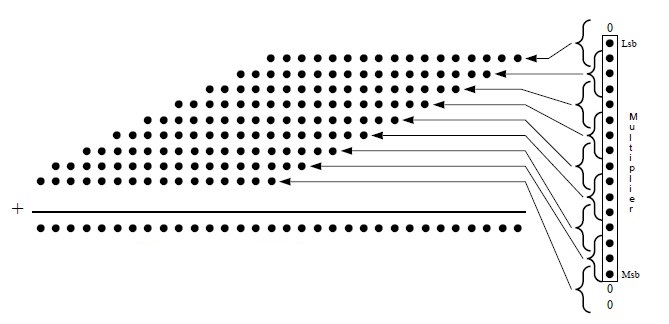
\includegraphics[width=.8\linewidth]{ {./schematic/wallace_standard.jpg} }
 %   \caption{}%\label{Fig:a}
  %\end{minipage}\hfill
%\end{figure}


\hspace{0.5cm}
\begin{figure}[htb]
\centering
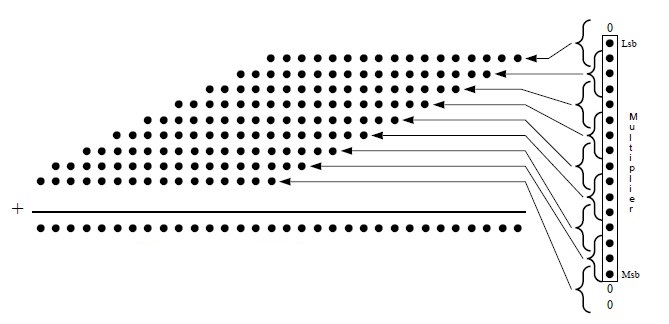
\includegraphics[height=6cm, width=\textwidth]{ {./schematic/wallace_standard.jpg}}
\end{figure}

\section{Partial Products Generation}
In order to obtain all the needed partial products, a simple 4-input multiplexer was implemented. It receives as inputs 0, a and 2a, and as selection bits the result of this
operation: $ (b_{2i} b_{2i-1}) xor (b_{2i+1} b_{2i+1})$ as shown in the following image. The $b_{2i+1}$ bit is also used as the sign of the partial product: if the result is negative,
the output of the multiplexer is negated in order to compute its 2's complement. 
% image
\hspace{0.5cm}
\begin{figure}[htb]
\centering
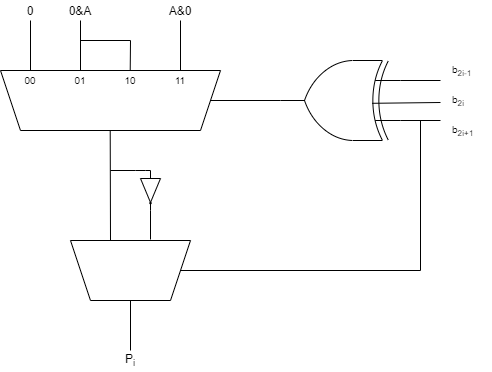
\includegraphics[height=6cm, width=\textwidth]{ {./schematic/Diagramma non titolato.png}}
\end{figure}

\section{Sign Extension}
The sign extension for unsigned multiplication is a technique that allows to reduce the number of redundant additions when computing the sum of the partial products.
In particular, when an operand is negative, the string of $'1'$ in the MSBs causes an unnecessary number of bits to be included in the final sum. The algorithm avoids this problem,
and also takes care of the $+1$ needed to compute the 2's complement without the need of an additional operation. The partial products are modified as shown in the following image,
where S is the sign of the operand. 
\hspace{0.5cm}
\begin{figure}[htb]
\centering
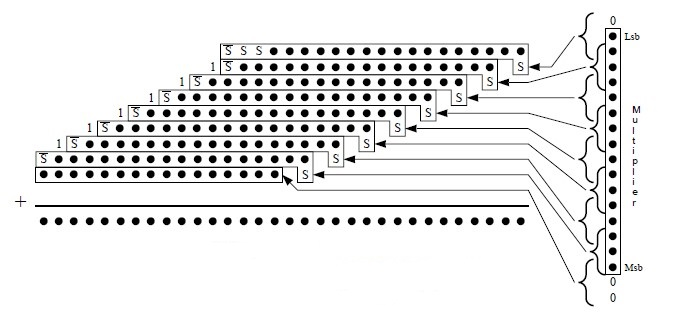
\includegraphics[height=6cm, width=\textwidth]{ {./schematic/wallace_signext.jpg}}
\end{figure}


\section{Dadda-Tree}
The final step for the computation of the result is to sum the partial products together. To compute this additions a Dadda adder was implemented. This component
achieves the solution by adding the operands by columns instead of rows. In particular, the Dadda implementation needs the number of rows to reduce to a specific value
each iteration; full adders and half adders are utilized to sum bits of the same column, thus reducing the number of rows. Contrary to the Wallace adder, the Dadda is
an "as late as possible" algorithm, meaning that the full and half adders are positioned as close as possible to the end of the operation. 
In order to visualize the positioning of the adders, schematics representing the operands were needed; the following picture is an example.
\hspace{0.5cm}
\begin{figure}[htb]
\centering
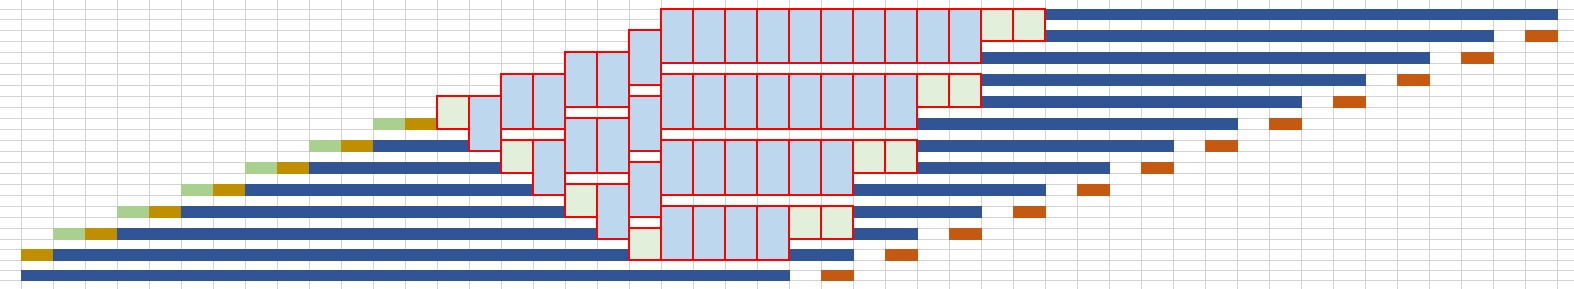
\includegraphics[height=6cm, width=\textwidth]{ {./schematic/stage_adder.jpg}}
\end{figure}


